
In order to experiment with different network architectures and exploit effects, it was necessary to reproduce each step in the process: 
Install AG suite (MulVal, XSB) $\rightarrow$ Define AG input model (Datalog/Prolog) $\rightarrow$ Generate AG (Java, C++, ANTLR4, sed) $\rightarrow$ Import NVD (JSON, XML $\rightarrow$ SQL) $\rightarrow$ Implement custom adaptor for Stochastic Model expected input (Python, inference) $\rightarrow$ Insert transition matrix into provided R script (ctrl+c, ctrl+v) 
After following this process precisely 2 times we understood why the AG based analytics community isn’t larger. Our immediate solution was to create a set of ansible roles and plays to automate the environment setup, test execution, and results collection entirely with a single command. This in itself lowers the barrier to entry for anyone interested in experimenting with attack graphs or looking to (quickly) reproduce our results.

\begin{figure}[ht]
\centering
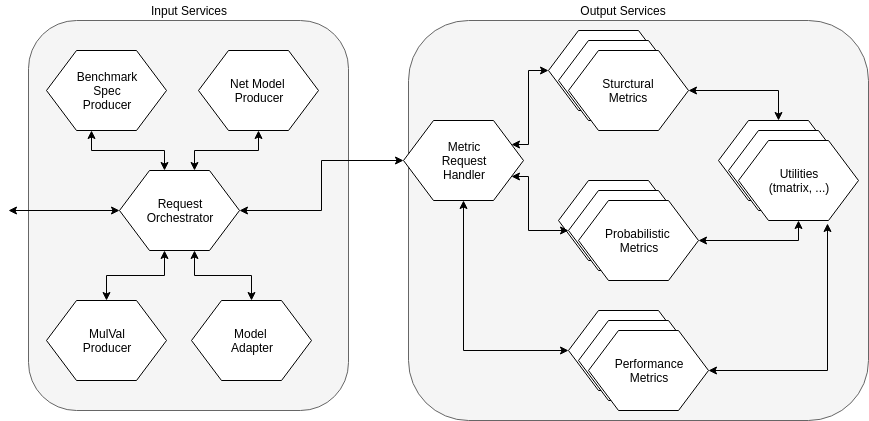
\includegraphics[width=.9\textwidth]{resource/img/ch_current/smaas/smaas_arch.png}
\caption{Security Metrics as a Service Architecture}
\label{fig:smaas:smaas_arch}
\end{figure} 


To handle the scale and volume of requests needed to support the advanced use-cases listed below, we are currently implementing and evaluating the following features in the SMaaS architecture:
Metric Isolation: Each metric should be independently deployable to allow scaling up and down as request volume dictates. Currently metrics are bundled in Python and R modules with logical separation at the function level.




